%%%%%%%%%%%%%%%%%%%%%%%%%%%%%%%%%%%%%%%%%%%%%%
\chapter{Esquem�ticos El�tricos}
\label{chapter:apendice_a}
%%%%%%%%%%%%%%%%%%%%%%%%%%%%%%%%%%%%%%%%%%%%
\begin{figure}[H]
	\centering
	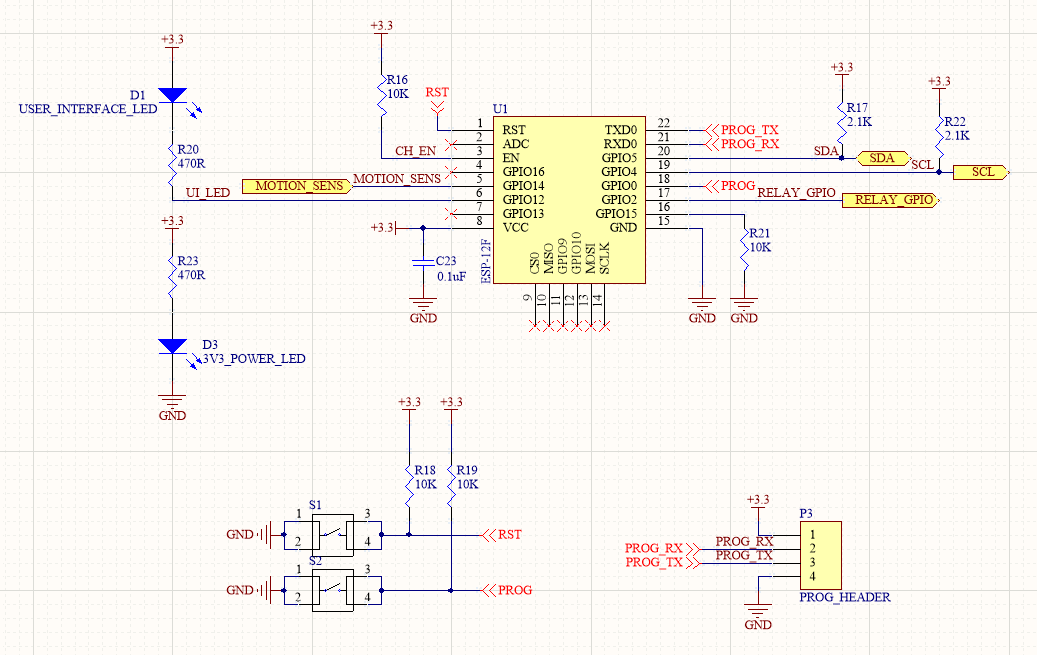
\includegraphics[angle = 90, width=0.65\columnwidth]{figuras/Schematic_Core_Processor}
	\caption{Esquem�tico el�trico referente ao microcontrolador.}
	\label{fig:Schematic_Core_Processor}
\end{figure}

\begin{figure}[H]
	\centering
	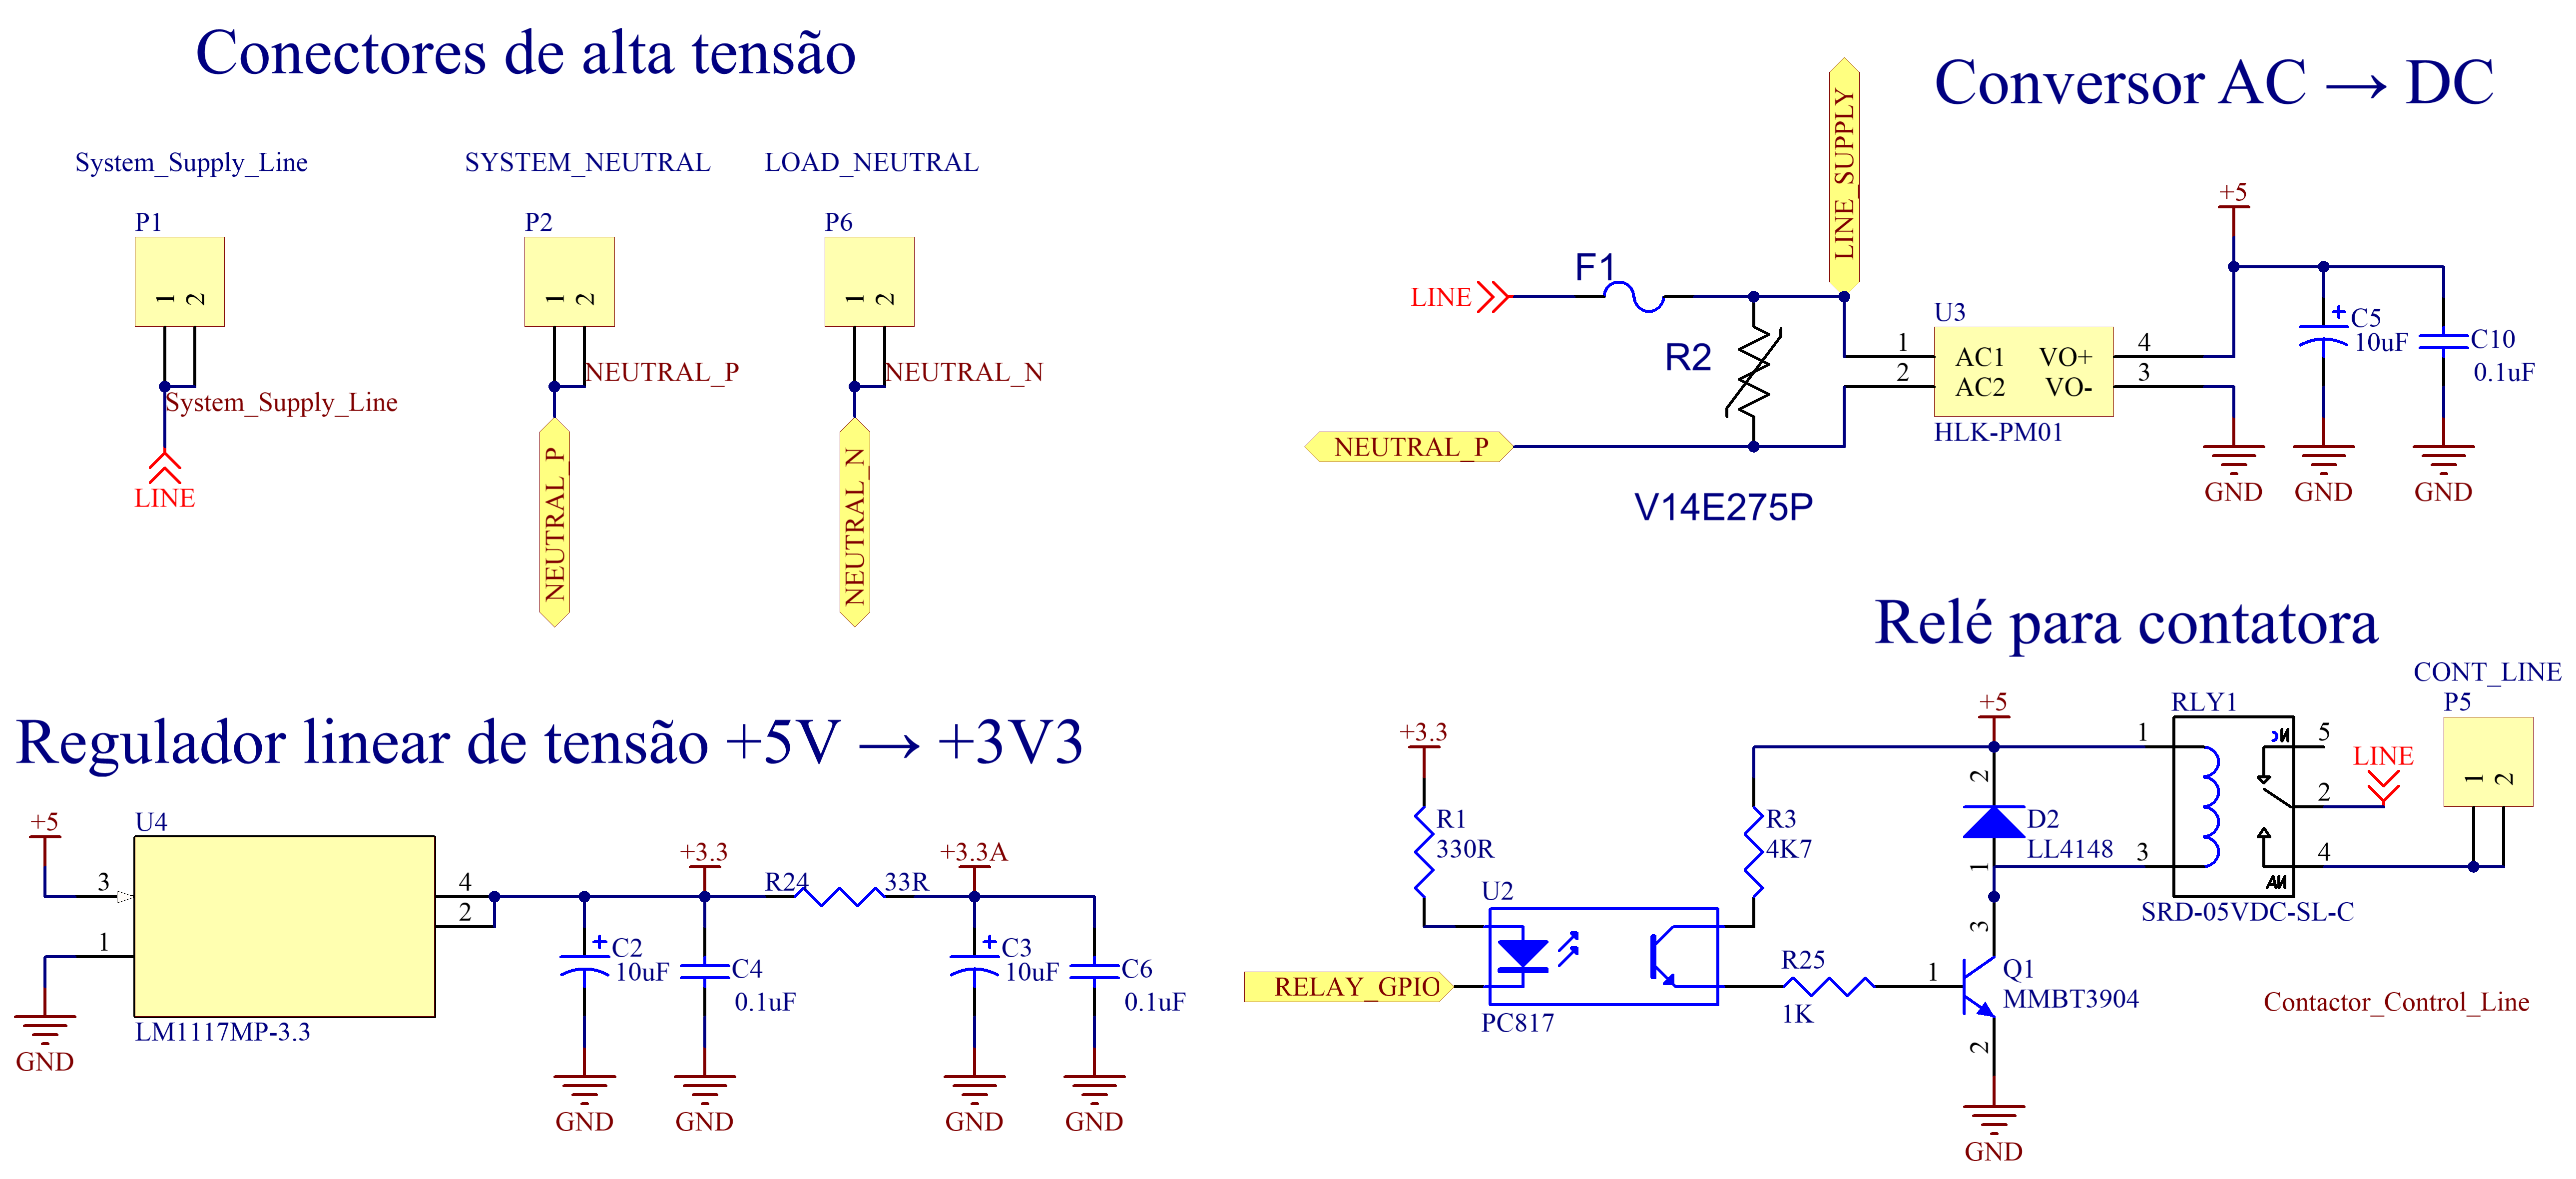
\includegraphics[angle = 90, width=0.8\columnwidth]{figuras/Schematic_Power_Supply}
	\caption{Esquem�tico el�trico da alimenta��o do circuito.}
	\label{fig:Schematic_Power_Supply}
\end{figure}

\begin{figure}[H]
	\centering
	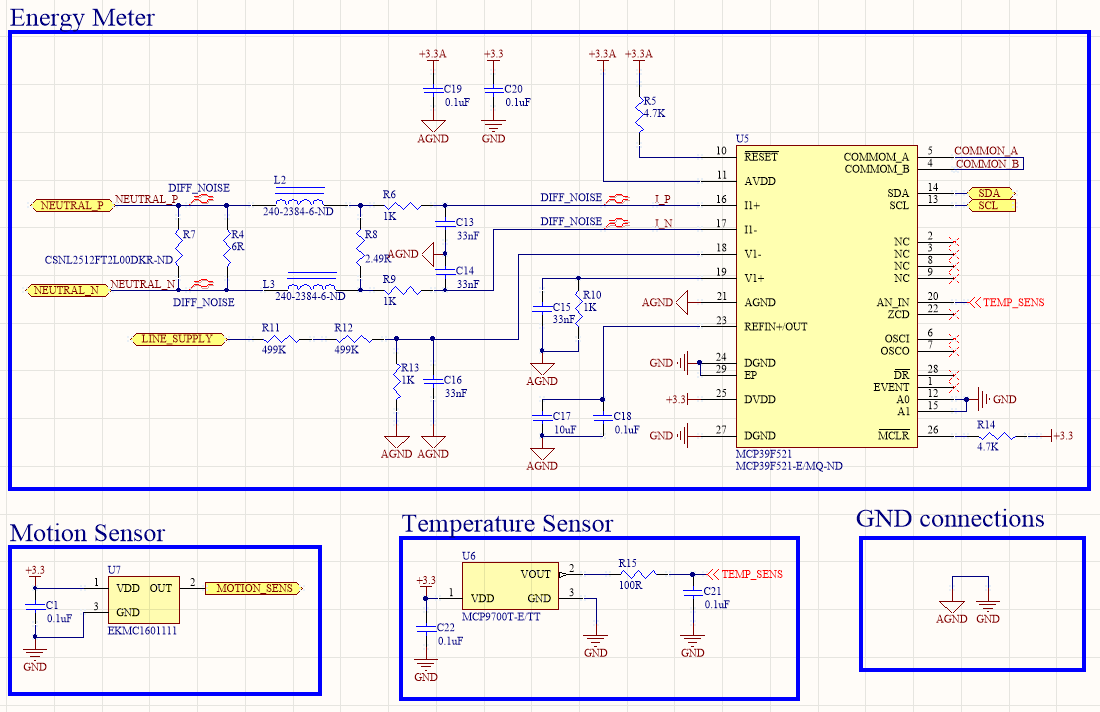
\includegraphics[angle = 90, width=0.9\columnwidth]{figuras/Schematic_Meter}
	\caption{Esquem�tico el�trico do sistema de medi��o da energia el�trica.}
	\label{fig:Schematic_Meter}
\end{figure}

\chapter{\textit{Layout} da PCB}
\label{chapter:apendice_b}
\begin{figure}[H]
	\centering
	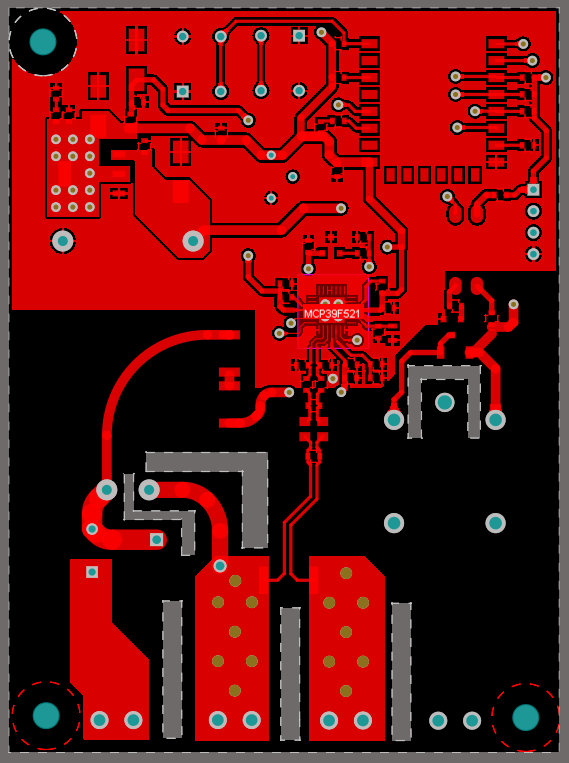
\includegraphics[width=0.8\columnwidth]{figuras/Layout_Top}
	\caption{\textit{Top Layer} do \textit{layout} da PCB.}
	\label{fig:Layout_Top}
\end{figure}

\begin{figure}[H]
	\centering
	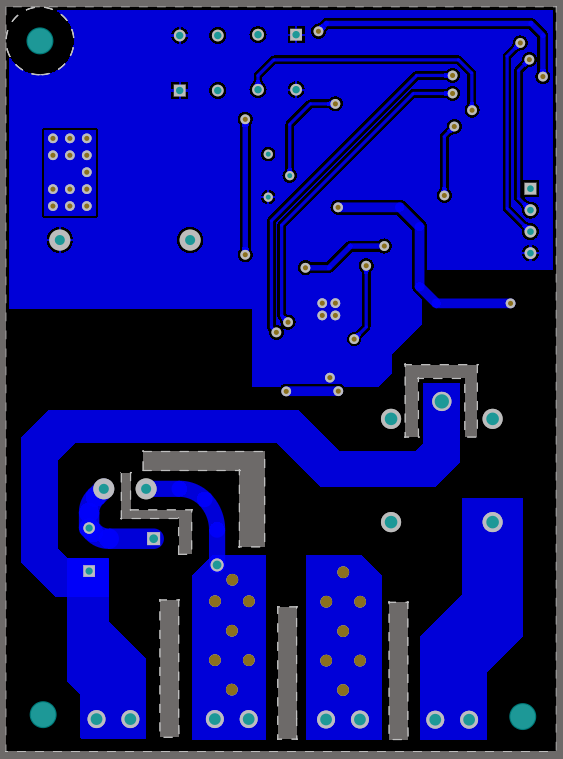
\includegraphics[width=1\columnwidth]{figuras/Layout_Bottom}
	\caption{\textit{Bottom Layer} do \textit{layout} da PCB.}
	\label{fig:Layout_Bottom}
\end{figure}

\begin{figure}[H]
	\centering
	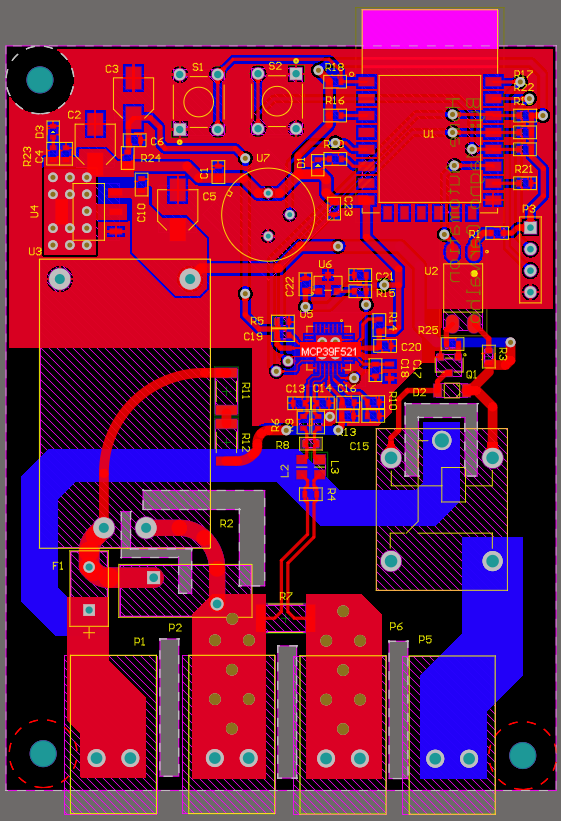
\includegraphics[width=1\columnwidth]{figuras/Layout_All_Layers}
	\caption{\textit{Layout} da PCB contendo os \textit{Layers Top} e \textit{Bottom}, os componentes e suas serigrafias.}
	\label{fig:Layout_All_Layers}
\end{figure}

\begin{figure}[H]
	\centering
	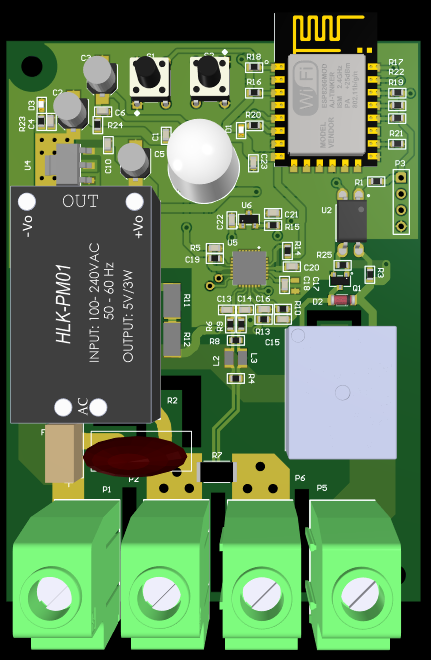
\includegraphics[width=1\columnwidth]{figuras/Layout_3D_Top}
	\caption{Vis�o superior da representa��o 3D do \textit{layout} da PCB.}
	\label{fig:Layout_3D_Top}
\end{figure}

\begin{figure}[H]
	\centering
	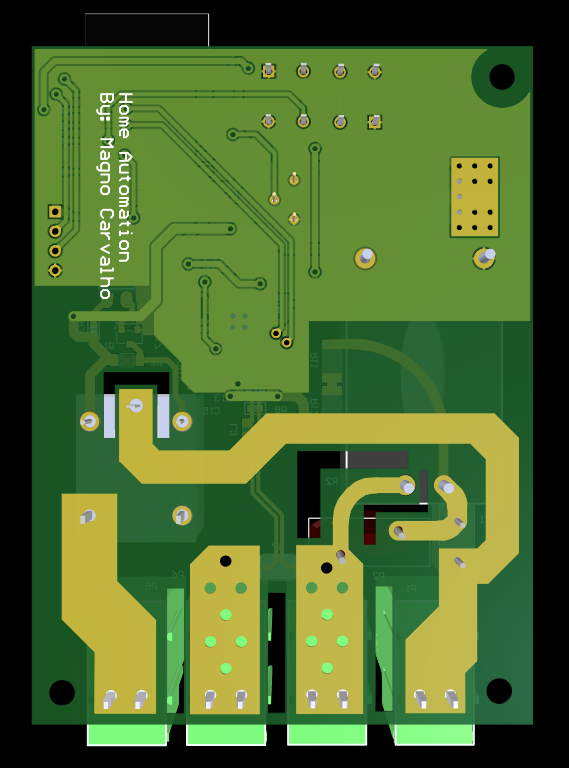
\includegraphics[width=1\columnwidth]{figuras/Layout_3D_Bottom}
	\caption{Vis�o inferior da representa��o 3D do \textit{layout} da PCB.}
	\label{fig:Layout_3D_Bottom}
\end{figure}

\begin{figure}[H]
	\centering
	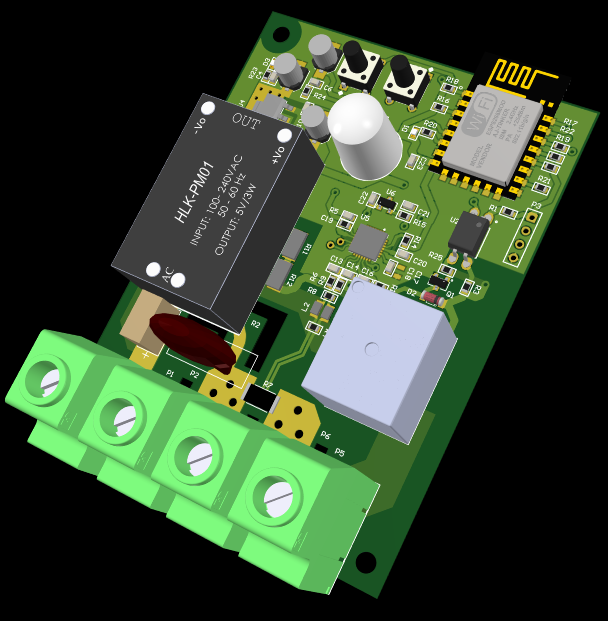
\includegraphics[width=1\columnwidth]{figuras/Layout_3D_Isometric}
	\caption{Vis�o isom�trica da representa��o 3D do \textit{layout} da PCB.}
	\label{fig:Layout_3D_Isometric}
\end{figure}

